\documentclass[tikz, border=12]{standalone}
\usepackage{stix, tikz, tkz-euclide, pgfmath}
\usetikzlibrary
	{
	intersections, decorations.markings, angles,
	quotes, calc, arrows, arrows.meta,shapes
	}


\usetkzobj{all}
%
\definecolor{blue}{RGB}{0,51,255}
\definecolor{green}{RGB}{0,153,0}
\colorlet{dcolor}{blue}
%

%
\tikzstyle{generic} = [thick,>={Stealth[scale=1.2]}]
\tikzstyle{angle} = [draw, To-To,angle radius = 20mm,   dcolor]
\tikzstyle{label} = [angle radius =20, dcolor]
\tikzstyle{parallel1} = [postaction={decorate, decoration={markings,mark=at position 0.5 with {\color{dcolor}\arrow{>}}}}]
%

%
\tikzset{pres/.code = {
\pgfgettransformentries{\mya}{\myb}{\myc}{\myd}{\mys}{\myt}
\pgfmathsetmacro{\preserve}{1/\mya}}}
%


\begin{document}
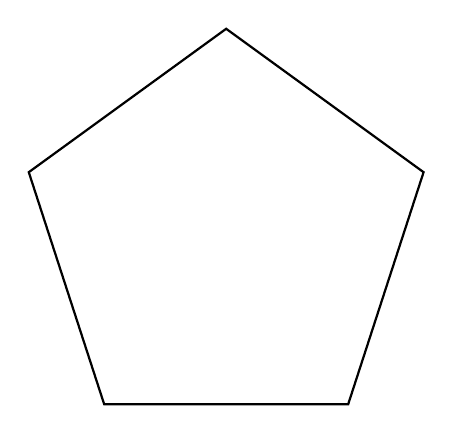
\begin{tikzpicture}
\scope[generic, pres]

\tkzDefPoint(0,0){A}

\node[draw, regular polygon, regular polygon sides=5,minimum size=150pt] at (0,0) {};
%
%
%

%

%
%
%
%
%
%


%
%
%
%
%
%
%

%


\endscope
\end{tikzpicture}
\end{document}